\documentclass{presentation}

\title{Soldering}
\subtitle{In the Chemistry Instrument Shop}
\author{Blaise Thompson}

\institute{University of Wisconsin--Madison}
\date{\today}

\begin{document}
\maketitle

\section{Introduction}

\begin{frame}{Introduction}
  Electronics Soldering
\end{frame}

\section{Surface Mount}

\begin{frame}{Surface Mount}
  text
\end{frame}

\begin{frame}{Capacitor}
  \centering
  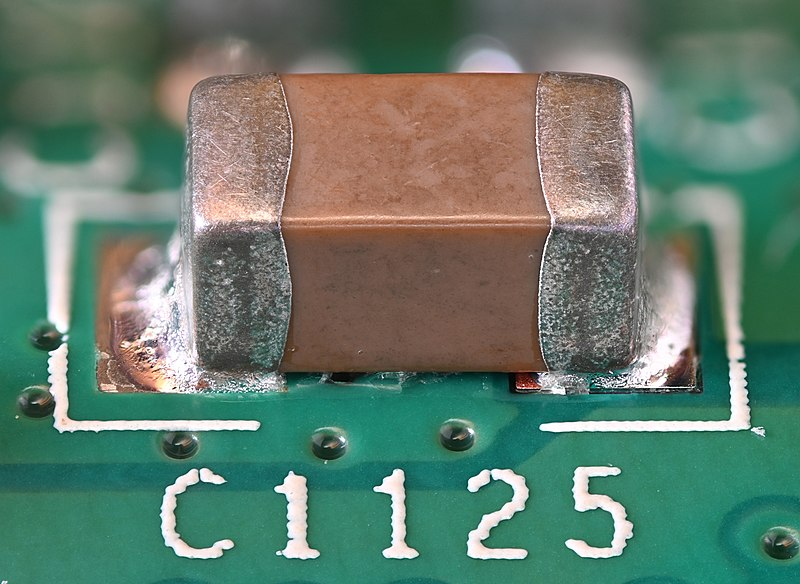
\includegraphics[width=\textwidth*3/4]{./Big_SMD_capacitor_2.jpg} \\
  \url{wikipedia:File:Big_SMD_capacitor_2}
\end{frame}

\begin{frame}{Reflow}
  youtube videos
  \begin{itemize}
    \item SMT \: Sample \#10 J-lead solder fillet forming 01
    \item 0603 SelfAlign
    \item 1005 Tombstone
  \end{itemize}
\end{frame}

\section{Through Hole}

\begin{frame}{Cold Solder Joint}
  \centering
  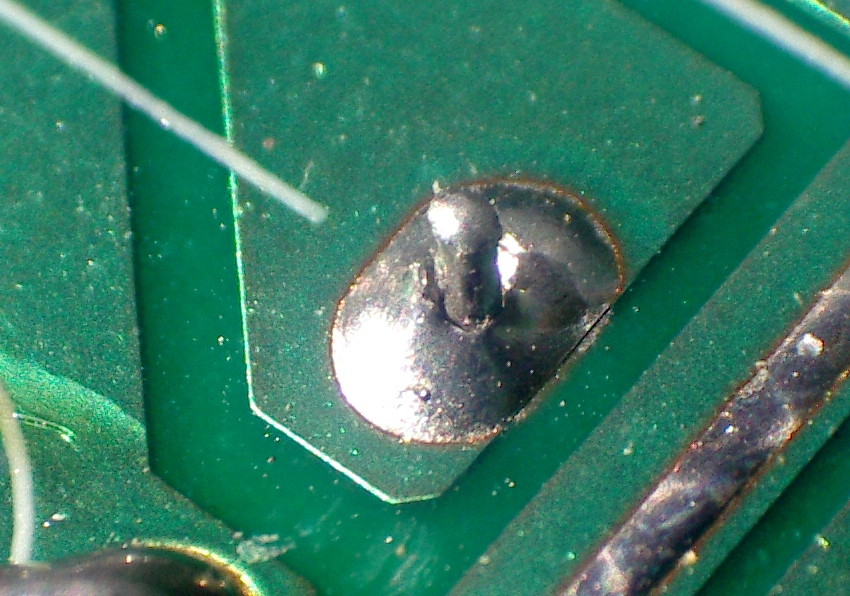
\includegraphics[width=\textwidth*3/4]{./Cold_solder_joint2.jpg} \\
  \url{wikipedia:File:Big_SMD_capacitor_2}
\end{frame}

\begin{frame}{Broken Joints}
  \centering
  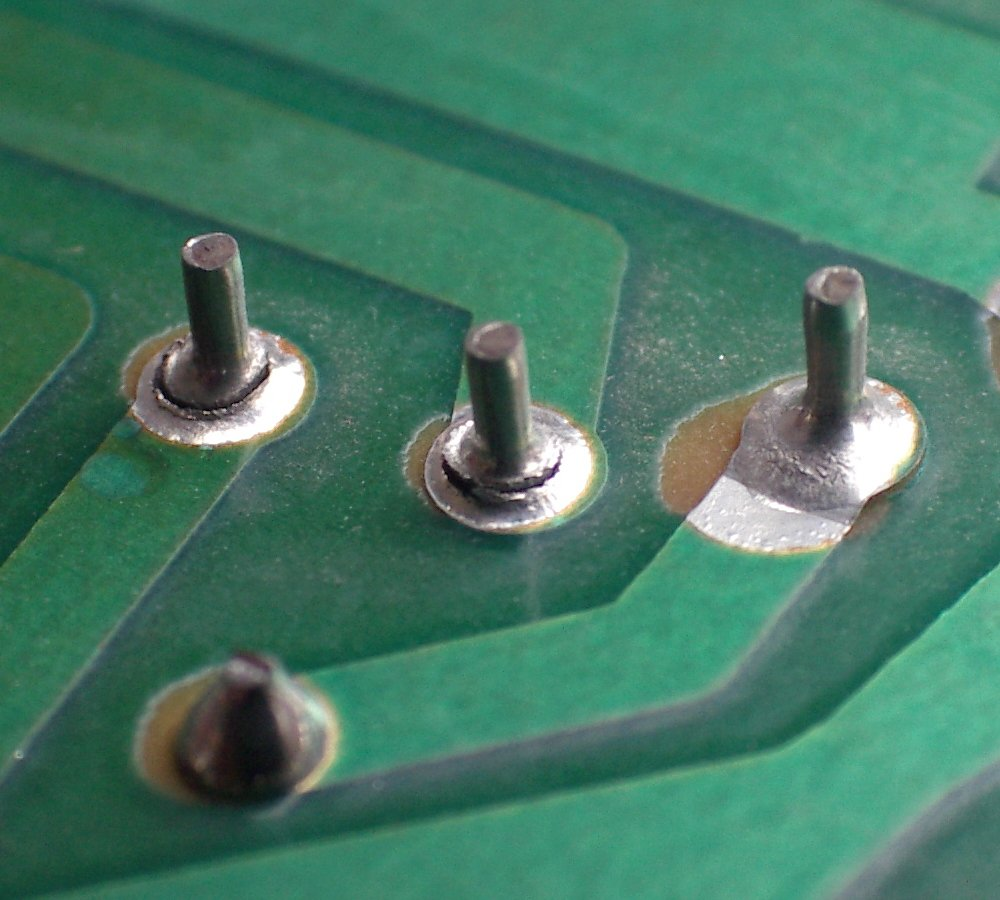
\includegraphics[width=\textwidth*3/4]{./Gebrochene_loetstellen.jpg} \\
  \url{wikipedia:File:Gebrochene_loetstellen}
\end{frame}

\section{Wire}

\begin{frame}{Wire to Board}
  Don't.
\end{frame}

\begin{frame}{Wire to Wire}
  Don't.
\end{frame}

\section{Desoldering}

\begin{frame}{Solder Tweezers}
  \centering
  \includegraphics[width=\textwidth*3/4]{./solder-tweezers.jpg} \\
  \url{wikipedia:File:Soldering_a_0805.jpg}
\end{frame}

\section{Conclusion}

\begin{frame}{Conclusion}
  Thanks for your attention!
\end{frame}

\end{document}
